\subsection{Opgave 11}
Figuren viser en trekant $ABC$.\\\\
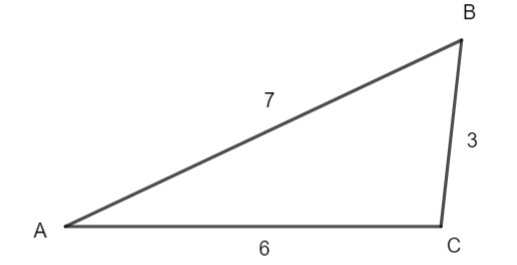
\includegraphics[width=10cm]{Opgave_11-20/Opgave_11/Opgave_11.jpg}

Følgende sidelængder er kendte: $|AB| = 7,\; |BC| = 3$ og  $|AC| = 6$.\\\\
Bestem vinkel $A$.\\\\


\ans
Da trekanten ikke er retvinkel kan vi bruge cosinusrelationen
\begin{align*}
    a^2 = b^2 + c^2 -2\cdot b\cdot c\cdot \cos(A)
\end{align*}
Her isolerer vi først cos(A)
\begin{align*}
    &a^2 -b^2 - c^2 = -2\cdot b\cdot c\cdot \cos(A)\\
    \Updownarrow \; &\\
    &\frac{a^2 - b^2 - c^2}{-2\cdot b\cdot c} = \cos(A)\\
    \Updownarrow \; &\\
    &-\frac{a^2 - b^2 - c^2}{2\cdot b\cdot c} = \cos(A)
\end{align*}
Nu indsætter vi sidelængderne på a,b og c's plads så $a = 3,\; b = 6$ og $c = 7$
\begin{align*}
    &-\frac{3^2 - 6^2 - 7^2}{2\cdot 6\cdot 7} = \cos(A)\\
    \Updownarrow \; &\\
    &-\frac{9 - 36 - 49}{84} = \cos(A)\\
    \Updownarrow \; &\\
    &-\frac{-76}{84} =  \cos(A)\\
    \Updownarrow \; &\\
    &\frac{76}{84} = \cos(A)\\
\end{align*}
Nu bruger vi den inverse funktion til cos altså arccos for at bestemme vinklen A
\begin{align*}
    A = \arccos\left(\frac{76}{84}\right) \approx 25.2 ^{\circ}
\end{align*}